\chapter{Tarea A}
\label{chapter:tarea_a}

En este apartado deberá segmentar los colores blancos y naranjas que aperecen en las imágenes disponibles en la carpeta \texttt{data}. Segmentar por colores es una técnica sencilla y útil en aplicaciones en las que se tiene un gran control sobre las condiciones de contorno: iluminación, tipo de objeto que se espera encontrar, color del fondo, etc. Para trabajar de forma eficiente, antes de empezar a procesar imágenes deberá definir algunos métodos. Estos métodos ya los utilizó en la 1ª sesión de laboratorio, así que aproveche estos pasos para afianzar.

\begin{figure}[h]
    \centering
    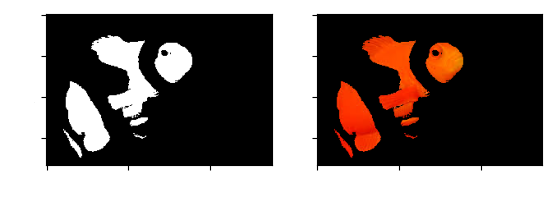
\includegraphics[width=0.5\textwidth]{Lab_2/template/figures/orange.png}
    \caption{Máscara y segmentación de colores naranjas.}
    \label{fig:orange_mask}
\end{figure}

\begin{figure}[h]
    \centering
    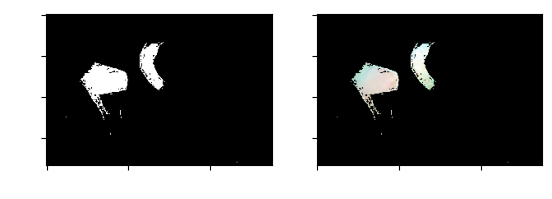
\includegraphics[width=0.5\textwidth]{Lab_2/template/figures/white.png}
    \caption{Máscara y segmentación de colores blancos.}
    \label{fig:whithe_mask}
\end{figure}

\begin{figure}[h]
    \centering
    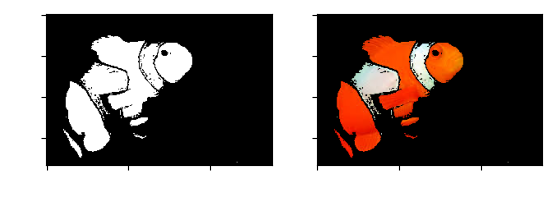
\includegraphics[width=0.5\textwidth]{Lab_2/template/figures/output.png}
    \caption{Máscara completa y segmentación del pez como combinación de colores blancos y naranjas.}
    \label{fig:fish_output}
\end{figure}